\documentclass{article}
\usepackage[utf8]{inputenc}
\usepackage{romannum}
\usepackage{amsfonts}
\usepackage{amssymb}
\usepackage{fancyhdr}
\usepackage{graphicx}
\usepackage{t1enc}
\usepackage{pdfpages}
\usepackage[magyar]{babel}
\usepackage[utf8]{inputenc}
\usepackage{amsmath}
\usepackage{mathtools}
\usepackage{pdfpages}
\usepackage{ marvosym } 
\usepackage{wrapfig}
\usepackage{hyperref}
\usepackage{pgfplots}

\pgfplotsset{width=\textwidth,compat=newest}
\hypersetup{
    colorlinks,
    citecolor=black,
    filecolor=black,
    linkcolor=black,
    urlcolor=black
}
\usepackage{romannum}
\usepackage{amsfonts}
\usepackage{amssymb}
\usepackage{fancyhdr}
\usepackage{graphicx}
\usepackage{t1enc}
\usepackage{svg}
\usepackage[magyar]{babel}
\usepackage[left=2cm,right=2cm,top=2cm,bottom=2cm]{geometry}

\title{Pályázat első negyedéves dokumentáció}
\author{}
\date{2}
\pagestyle{fancy}
\lhead{X pályázat első negyedéves jelentés}
\rhead{ACSG Kft.}
\cfoot{\thepage. oldal}

\begin{document}
\pagenumbering{arabic}

\maketitle
%
\includegraphics[b]{acsg.svg}
\thispagestyle{empty}
\setcounter{page}{0}




\newpage
\tableofcontents
\newpage
\section{Cégünk bemutatása}
Üzemünk Győr szívében, közel a belvároshoz, és az osztrák, szlovák határhoz, az autópályától nem messze található, így rendkívül jól megközelíthető. Cégünk 2005-ben alakult. Fő tevekénységi körünk a kábelkonfekcionálás és részegység összeszerelés.\vspace{10pt}\\
Elsősorban nagy bonyolultságú termékeket, kis és közepes darabszámban, precíz, ellenőrzött gyártási körülmények között, 100 $\%$-os elektromos ellenőrzéssel gyártunk. Emellett vevőinknek segítünk a termékeik fejlesztésében, optimalizálásában mind a technológia mind a felhasznált alapanyagok tekintetében. A tulajdonosok a mai napig aktív résztevői a cég működésének.\vspace{10pt}\\
A cég sikerének egyik alapja, hogy nem csupán bérmunkával foglalkozik, mint a konkurensek nagy része, hanem egyedi megoldásokat fejleszt vevői részére. Folyamatosan integrálva az új, innovatív gyártási technológiákat, ezzel növelve a hatékonyságot.\vspace{10pt}\\
Az évek során folyamatosan növekvő vevőkörre és árbevételre tudtunk szert tenni. Fejlődésünk töretlen, 2018-ban elkészült az új, saját tulajdonú üzemcsarnokunk is. A közel 4000 $\text{m}^2$ területünk lehetővé teszi számunkra még több vevő kiszolgálását, új technológiák implementálását, munkahelyek bővítését, kapacitásnövelést.\vspace{10pt}\\
Több mint 120 munkatárssal dolgozunk együtt, akiknek folyamatosan biztosítjuk a szakmai fejlődését.\vspace{10pt}\\
Folyamatainkat egy modern, nemzetközi vállalatirányítási rendszerben kezeljük, az árajánlatadástól kezdve, a dokumentumkezelésen, a beszerzésen, a gyártáson, a logisztikán keresztül a könyvelésig bezárólag.\vspace{10pt}\\
Ezen előnyöket kihasználva az ACSG nemcsak egyedülálló, de egyben a leghatékonyabb cég is a kábelkonfekcionálás területén.
\begin{figure}[h]
    \centering
    %\includegraphics[]{ceg_kep.png}
    \caption{ACSG telephely fotó, Győr}
\end{figure}\\


\newpage
\section{Első negyedéves munka összefoglalása}
A pályázat első negyedévében fő feladatunkként azt tekintettük, hogy a jelenlegi rendszerünk teljeskörű felmérését elvégezzük annak előnyeivel és hátrányaival együtt
, továbbá a továbbfejlesztési lehetőségeket, irányvonalakat minél szélesebb spektrumban megvizsgáljuk.\vspace{5pt}\\
Kiemelten fontosnak tartjuk, hogy végleges megoldásunk kellően újszerű, innovatív technológiai elemeket, megoldásokat tartalmazzon, precíz, biztonságos, termelékeny, későbbiekben továbbfejleszthető, rugalmas legyen, így mérnökeink kellő szakmaisággal, legjobb tudásuk szerint dolgoznak a projekten.\vspace{5pt}\\
A továbbiakban az egyes fejezeteknek megfelelő bontásban kerülnek részletezésre a pályázathoz tartozó kutatásfejlesztés főbb aspektusai.

\section{Jelenlegi rendszer}
\subsection{Ismertetés}
Gyártórendszerünk egy JN07SD-IS-C típusú krimpelő és illesztő gép. Kábelek krimpelését és 
házazását tudja elvégezni, részletes dokumentációja és képek a mellékletek közt találhatóak meg.\\
A teljesség igénye nélkül a projekt szempontjából fontos megemlíteni a következő aspektusait a 
cellának:
\begin{itemize}
    \item A krimpelő és házazó rész (később mechanikai rész) mechanikailag függetleníthető az adagolórendszer(ek)től.
    \item A cella kábelházakkal történő töltése fix mechanikus módon történik, minden eges háztípushoz speciális
    fészek és adagoló szükséges.
    \item A kábelszínek megkülönböztetésén és az alapvető biztonsági, funkcionalitást biztosító szenzorokon kívül egyéb adatgyűjtő berendezést nem tartalmaz.
    \item IoT felszereltséggel nem rendelkezik.
\end{itemize}
A működésről a gyártó oldalán megtekinthető egy \href{https://www.youtube.com/watch?v=biwFZ-rbG8k&t=0s}{\textbf{Videó}}.\vspace{5pt}\\
Rövid leírás:\\
Az adagolóba helyezett dobról folyamatos kábel lehúzás történik,
ezeket méretrevágja a gép, illetve krimpeli, ónfürdőbe meríti majd a megfelelő házba helyezi és a kész 
terméket egy gyűjtőbe ejti.

\subsection{Probléma}
Jelenlegi rendszerünk a tömegtermelésre, milliós darabszámú gyártásra optimalizált,
a kisszériás, gyakori átállást igénylő gyártás esetén, amely cégünknél gyakran előfordul,
egy-egy termékből adott esetben csak pár százas nagyságrendű gyártásra van szükségünk, de egy nap
akár a százas nagyságrendet is elérheti a különböző terméktípusok száma. Tekintve a mechanikai
kiszolgálórendszer kötöttségét egy-egy termékváltás sem időben, sem anyagi vonzatban nem 
térül meg.\\
Továbbá az IoT standardek sem biztosítottak, ami igen nagy hátrányt jelent egy-egy kisebb
üzemi egység teljes felügyeleti rendszerbe történő beágyazásánál.\\
Belátható, hogy ezen problémák áthidalásához a gép egyes részegységeit át kell alakítani,
szenzorokkal kell bővíteni, illetve szotfveresen is igen nagy változtatásokat kell eszközölni.


\newpage
\section{Célkitűzés}
A kutatásfejlesztési feladat elsődleges célkitűzése az optimális megoldás megtalálása a jelenlegi rendszer problémáinak kiküszöbölésére, a gyártócella ipar 4.0-ba való integrálása, termelékenységének növelése, üzemeltetési költségeinek csökkentése, bizonságtechnikai fejlesztése minőségi mérnöki szaktudással, mindezt a fejlesztési költségkeretben tartva a felmerülő költségeket.\vspace{5pt}\\
A mérnöki munka során kifejezetten fontos, hogy a kérdéskört minél több nézőpontból, minden egyes aspektust kellő körültekintés mellett megvizsgáljunk, mérlegeljünk, továbbá a megfelelő kutatások megismerése, tanulmányozása, a projekt dokumentáció során való mellékelése kiemelt fontossággal bír. Nem elegendő csupán a meglévő mondhatni standard, bevett megoldások használata, hiszen minden mérnöki feladat specifikus, főként
az ilyen komplex rendszerek vizsgálata, melyeknél nagy fontossággal bír a gyakorlati megvalósíthatóság, működési hatékonyságon túl a stabil elméleti háttér, továbbá az egyes mérnöki specifikációk egymást támogató integrálása, koollaborációja. Az innováció a kutatásfejlesztésben elengedhetetlen, nincs ez másképp jelen esetben sem, végleges megoldásunk megtalálása során törekszünk arra, hogy a lehető legújabb kutatások eredményeiből okulva
 és természetesen a már kiforrt régebbi kutatási, elméleti eredmények segítségével lehetőleg új metódussal sikerüljön rendszerünk esetében megvalósítani a kitűzött fejlesztési célokat.\vspace{5pt}\\
A feladat során a következő célkitűzések fogalmazhatóak meg:
\begin{itemize}
    \item A mechanikai adagolórendszer lecserélése rezgőtárcsás adagolóra, illetve robot manipulátorra. 
    \item Az új adagolórendszer teljesen autonóm működéső legyen, megfelelő biztonsági automatikákat is tartalmazza
    \item A rendszer különálló autonóm, jól elkülöníthető részekre legyen felbontható
    \item A rendszer egy alrendszere képes legyen tetszőleges csatlakozó házakat valós időben detektálni a munkaterületen, ezeket klasszfikálni és megfelelő adatot szolgáltatni a manipulátornak, hogy azokat biztonságosan minimális kontaktidővel a fészekbe tudja juttani
    \item A detektáló alrendszer kizárólag kamerából (detektor) származó képekből oldja meg feladatát, más szenzor nem használható ezen részben
    \item A detektáló alrendszer minimum öt különböző csatlakozó házat meg tudjon különböztetni
    \item Az egyes csatlakozó házak hozzáadása, elvétele, könnyű, minimális számítási kapacitást és időt igénylő legyen
    \item A rendszer rendelkezzen egy többféle eszközről lokálisan és interneten keresztül elérhető felhasználói felülettel, melyen keresztül metaadatok kérdezhetők le, logok hívhatók elő, a beavatkozó szervek kezelhetők, továbbá frissíthető az aktuális munkaciklus beállításai beleértve a detektáló rendszer frissítését
    \item Valós időben szükséges egy az egész folyamatot monitorozó, kinyert adatok alapján mesterséges intelligencia alapú optimalizációs alrendszer, mely előrejelzést ad a termelékenységre, esetleges hibákra, selejt rátára, továbbá instrukciókkal látja el a felhasználót, hogy hogyan tud növelni a kihozatal mennyiségén, esetlegesen minőségén
    \item Amennyiben lehetséges szimulációs opciók, keretrendszerek implementálása is történjen meg, hiszen így a valóságban elég finomhangolni, tesztelni, gyorsabb lesz a fejlesztés, más projekteknél is felhasználható egy univerzális szimulációs keretrendszer
    \item Kutatási célzattal szeretnénk implementálni deep reinforcement learning, illetőleg GAN alapú megoldásokat, melyek alkalmazása jelenleg az iparban a többi megoldáshoz képest csak korlátozottan terjedt el, azonban elméleti eredményeik kiemelkedőek
    \item A kutatási eredmények megfelelő dokuemntálása és későbbiekben való felhasználása is céljaink közt szerepel
\end{itemize}
\newpage
\section{Átalakítási tervek}
A feladatot célszerű már a tervezés folyamatában alrendszerekre bontani, melyek egyenként önálló működésre képesek, ez igen nagy segítség tud lenni az egyes működések szimulációjánál, optimalizálásnál, a teljes komplex rendszer összeillesztésénél. Ennek megfelelően az alábbi részrendszerek kerültek elkülönítésre, melyek fejlesztése párhuzamosan is végezhető:
\begin{itemize}
    \item Objektum detektáló alrendszer: feladata a manipulátor alrendszernek általánosított koordinátákat küldeni, melyek segítségével az objektum megfogása megvalósulhat (természetesen ebbe beletartozik a klasszifikáció is)
    \item Objektum manipuláló alrendszer: feladata a detektáló alrendszerből kapott adatok segítségével a fészekbe juttani a csatlakozó házakat
    \item Optimalizációs alrendszer: feladata az egész rendszerre kiterjedő predikció, optimalizációs instrukciók kiadása, végrehajtása
    \item Biztonsági alrendszer: feladata a mindne körülmények közötti mindenkori biztonsági faktor megteremtése
\end{itemize}
A dokumentáció későbbi szakaszában ezen alrendszerekhez kapcsolódó tervek, elvárások részletezésre kerülnek.\vspace{5pt}\\
Általánoságban elmondható, hogy minden fizikai részét a gyártócellának digitalizálni szeretnénk különböző szenzorok és mikrovezrélők segítségével, hiszen ha sikerül a főbb elemekről megfelelő információt gyűjtenünk, úgy egy teljeskörúen funkciónáló digitális iker (digital twin)
hozható létre a celláról, mely megkönnyíti a valós rendszerre való implementálását egyes változtatásoknak, szimulációs, tesztelő lehetőséget biztosít, továbbá a kontrol részt is nagyban segíti, elegánsabb és valósághűbb megoldást kaphatunk így.\\
\begin{figure}[h]
    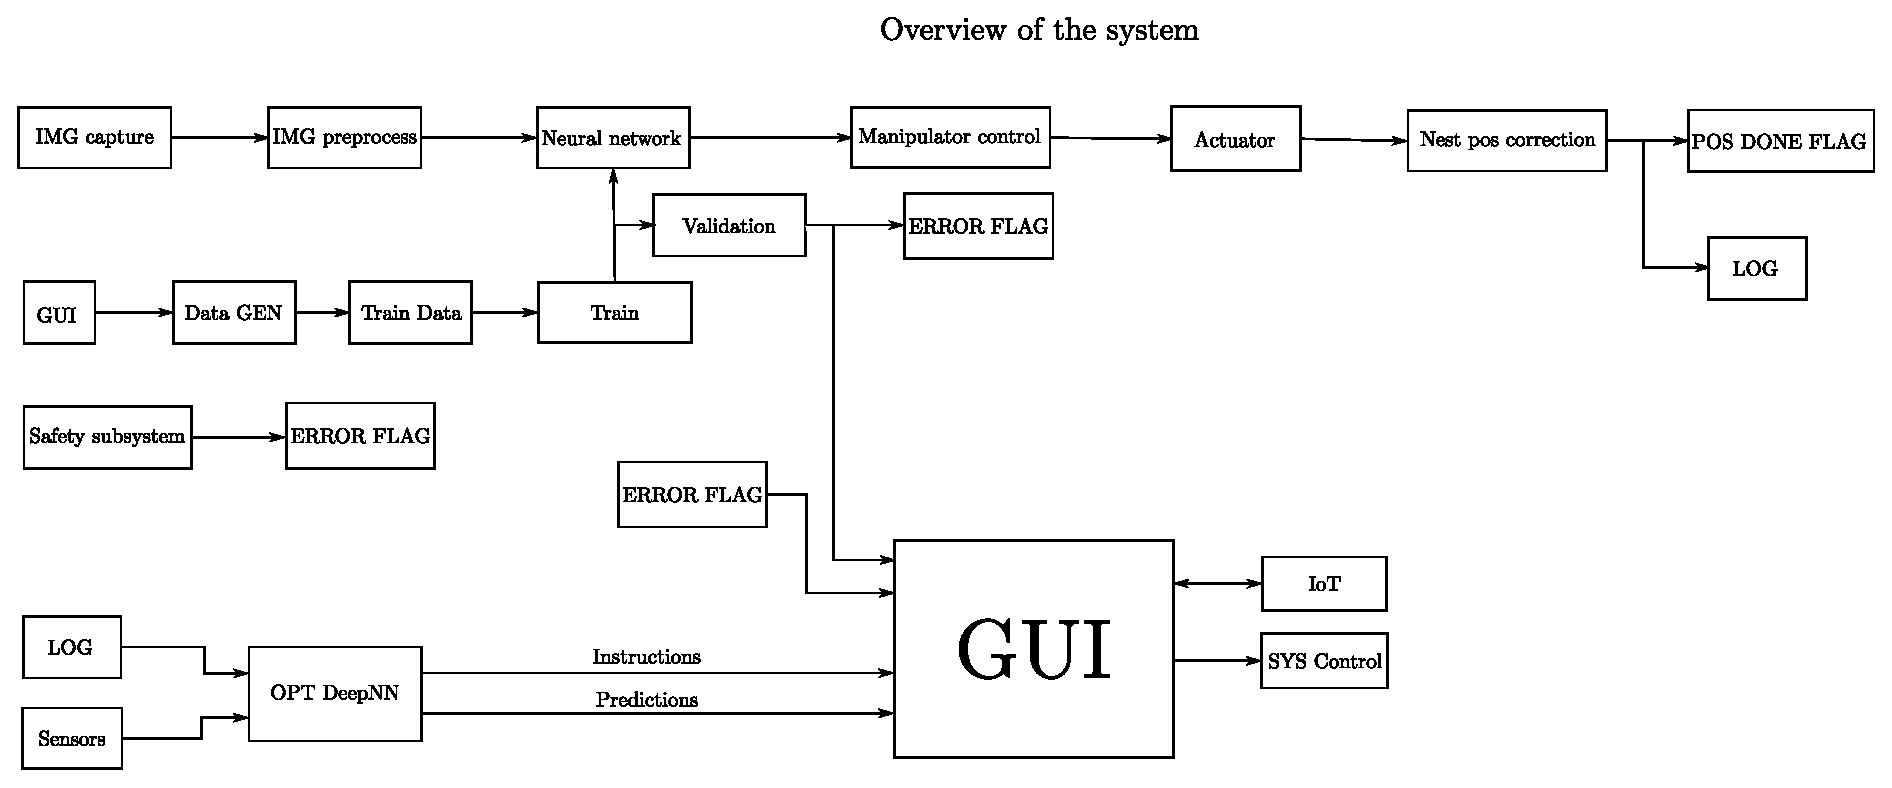
\includegraphics[scale = 0.6]{system_overview.eps}
    \caption{Tervezett rendszer vázlat}
\end{figure}
\newpage
\section{Objektum detektáló alrendszer}
\subsection{Működés összefoglalása, követelmények}
Az alrendszer egyrészt fizikai részből áll, mely egy kamerát, illetve az abból kinyert kép feldolgozását végző hardverből áll.
 Másrészt a komplexebb részét a szoftveres háttér képzi, mely a nyers képből előfeldolgozást követően mesterséges intelligencia módszerekkel megállapítja azon általános koordináták halmazát, melyeket átad az objektum manipuláló rendszernek.\vspace{5pt}\\
Követelmények: kizárólagosan a detektorból érkező képet használhatja az alrendszer, valós időben kell működnie, legalább öt különféle csatlakozó ház megkülönböztetésére képesnek kell lennie, könnyű változtathatóság és minimális számítókapacitás, illetve számítási idő kell jellemezze
az egyes átállásokat objektumok között.\vspace{5pt}\\
 \textbf{K+F feladat:} alrendszer optimalizálása a követelményekhez és lehetőségekhez.
\subsection{Szenzor és feldolgozó egység}
Mivel a projektleírás leszögezi, hogy az objektumok detektálása, pozíció- és orientációmeghatározása
kizárólag kamerákból (detektor) kapott képek alapján történhet, a feladat ezen részéhez semmilyen
más szenzorból kapott adat nem használható, így kiemelten fontos a megfelelő hardver
kiválasztása. A detektor esetében először is az alapvető paraméterek (látószög, fókusztávolság, felbontás stb.),
 majd ezt követően a használt hullámhossz, színtartomány, FPS (frame per second) meghatározása szükséges.
 Fontos megvizsgálni több lehetőséget is, hogy megfelelő bizonyossággal válasszunk kamerát.
 Egy másik aspektus a feldolgozó egység, mikroprocesszor, melyen majd a különböző képmanipulációs
 tevékenyéget végezzük, itt szintén méreteznünk kell és a szükséges teljesítménynek megfelelő
hardvert használnunk.\vspace{5pt}\\
\textbf{K+F feladat: }A projekt kívánalmainak megfelelő detektor és posztprocesszor egység kiválasztása.
\subsection{Előfeldolgozás}
A neurális hálóba való betöltés előtt célszerű valamilyen előfeldolgozást (preprocesszálás)
végezni a detektorból származó nyers képekkel, ez lehet páldául zajszűrés, méretre vágás, skálázás
szegmentálás, élesítés. Ezen műveletek egyszerű képfeldolgozási algoritmusok, metódusok
segítségével valósíthatóak meg.\vspace{5pt}\\
\textbf{K+F feladat: }Az adott neurális hálóhoz illeszkedő preprocesszáló egység létrehozása
hardveresen és szoftveresen.
\subsection{Klasszifikációs és szegmentáló neurális háló}
A képfeldolgozást egy mély neurális háló segítségével szeretnénk megvalósítani, mely napjainkban
igen elterjedt, a modern képfeldolgozásban az ilyen megoldások úttörőnek számítanak és 
legtöbbször komplex és egyszerű feladatokban is felülmúlják az egyéb módon működő társaikat.\\
Alapvetően két járható út lehetséges az objektumok detektálásánál, az egyik, hogy az egész
munkaterületről készített képet kisebb képekre bontjuk, melyeken egy-egy specifikus elem
látható, majd ezeket klasszifikáljuk és állapítjuk meg pozíciójukat és orientációjukat. A
másik opció, hogy az egész képet szegmentálva a megfogási pontokat hőtérképszerűen állapítjuk meg,
majd ezen pontok közül választ az algoritmus. Természetesen a két módzser közt van átfedés 
és több vegyes megoldás is alkalmazható.\\
Több már kipróbált objektum detektáló deep learningen alapuló háló, keretrendszer és algoritmus
létezik (pl.: U-net, Trans-U-net, YOLO) ezek vagy hozzájuk hasonló architektúrák vizsgálata,
tesztelése, az eredmények összehasonlítása a kutatásfejlesztés szerves részét fogják képezni.\\
Kifejezetten fontos esetünkben a háló bővíthetősége, hiszen egy-egy objektum hozzáadása a
rendzserhez szükséges a gördülékeny, gyors átállásokhoz a munkacellában, erre egy lehetséges megoldás 
lehet aggregált neurális hálókat alkalmazni.\\
\textbf{K+F feladat: }különböző háló architektúrák vizsgálata, ötvözése, optimalizálás.
\subsection{Háló(k) tanítása}
Az egyes hálóarchitektúrákon túl igen fontos aspektusai vannak egy-egy ilyen rendszernek.
Egyrészt a hiperparaméteroptimalizálás korántsem triviális, hiszen a szuboptimális megoldás jósága
vagy egyáltalán létezése nagyban függ tőle, ennek optimalizálására teljeskörű matematikai
tézis nem létezik, csupán a gyakorlatból tapasztalati úton szerzett praktikák, ajánlások léteznek, így
ebben a témában is nyitott kérdésekkel találkozhatunk, melyekhez nagyszámú háló tanítást
kell végeznünk. Másrészt a rendelkezésre álló adatok milyensége is megkerülhetetlen és folyamatos
monitorozást igényel a fejlesztés során, hiszen zajos vagy hibás adat miatt teljesen rossz
megoldásokat kaphatunk szinte észrevétlenül.\vspace{5pt}\\
\textbf{K+F feladat: }Az időkeretben maradva minél több háló kialakítás minél többszöri tanítása,
hiperparaméteroptimalizálás, következtetések levonása.
\subsection{Adatszerzés}
A mesterséges intelligencia tárgyalásában, illetőleg rengeteg más területen is kimondható, hogy
az adat a kulcs, az elengedhetetlen fundamentuma ezen tudományágaknak és gyakorlatbeli alkalmazásoknak.
Ennek megfelelően gyűjtése, osztályozása, címkézése, rendszerezése, szűrése kiemelt jelentőséggel bír.\\
Jelen projektnél azonban azzal a kihívással is szembe kell néznünk, hogy a valós környezetből
származó adatok esetében a költségek mint idő- és pénzbeli aspektust tekintve igen magasak, erőforrásigényesek.
Ennek kiküszöbölése érdekében a tanításhoz használt adatainkat szintetikusan szeretnénk generálni,
majd a feltanított modellt valós környezetbeli képekkel validálni, illetve amennyiben a struktúra
lehetővé teszi illeszteni a fizikai környezetre további tanulási ciklusokkal.\vspace{5pt}\\
\textbf{K+F feladat: }Valóságot tükröző szintetikus adatgenerálás minimális számítási idővel és teljesítményszükséglettel.
\subsection{Alrendszer kimenete}
Fontos megemlíteni, hogy a manipuláló alrendszer csakis a lépfeldolgozó, objektum detektáló
részből kap információt, azaz koordinátákat, orientációt, sorrendiséget.

\section{Objektum manipuláló alrendszer}
\subsection{Működés összefoglalása, követelmények}
Az objektum manipuláló alrendszer elsődleges feladata a munkaterületen lévő elemek biztonságos
felvétele majd adott tűréssel a fészekbe helyezése. Ehhez szükséges minden adatot kizárólagosan az objektum
detektáló alrendszer biztosít számára.\\
Követelményként elsősorban a precíz és gyors működés elvárt, továbbá természetesen mindezek mellett
semmilyen káreset nem történhet.\\
\textbf{K+F feladat: }Több lehetőség tesztelése az alrendszer működése, kialakítása kapcsán.
\subsection{Manipulátor}
Tekintve a szükséges flexibilitást mindenképp valamilyen robotmanipulátorra van szükséges
a feladat teljeskörű elvégzésére. Számtalan kialakítású robot létezik és alkalmazható, számunkra
humanoid (RRR) vagy SCARA (RRT) a legalkalmasabb tekintve a viszonylag kis munkaterületet és
a megfogni kívánt objektumok variációjának skáláját. A humanoid robotkar előnye, hogy tetszőleges
orientációban és irányból képes végrehajtani feladatát, viszont ezen előny kellően komplexszé is teszi
a procedúrát. A SCARA legfőbb pozitívuma a nagy munkasebesség, melyet nagy pontosság és stabilitás
támogat, hátránya azonban, hogy hengerrel közelíthető munkaterülete, illetve komplex 3D forgatásra nem képes, azt
csak síkban tudja végrehajtani. Továbbá a végegység milyensége is kérdéseket vet fel, hiszen
tüskés villától a vákuum ejektoron át a teljesen egyedi többállású megfogó is alkalmazható.\vspace{5pt}\\
\textbf{K+F feladat: }Optimális robotmanipulátor és végegység keresése, tesztelése.
\subsection{Irányítási keretrendszer}
A manipulátorok irányítása azon túl, hogy felhazsnálófüggetlen kell legyen, azaz teljesen
autonóm rendszerre van szükségünk, lehetőséget kell biztosítani az intuitív jellegű manuális kezelésre is.\\
Az automata rész az előző alrendszertől kapott adatstruktúra felhazsnálásával
inverz kinematikai számítások útján pályát tervez az objektum felvételéhez, továbbá
a különböző szenzorok által szolgáltatott jeleket feldolgozásával a lehetséges hibákat
korrigálja a szabályozás.\\
Napjaink rendszereinél elvárás, hogy a fizikai folyamatot virtuálisan is nyomon lehessen követni,
az aktuális folyamatjellemző értékeket valós időben is látni, továbbá az aktuátorokat irányítani lehessen.
Ezen célok kielégítésére egy digitális ikert szeretnénk megvalósítani, mely elérhető a 
felhazsnálói felületen keresztül és a rendszerrel kapcsolatos fentebbi követelményeket
teljes mértékben kielégíti.\\
Egy célszerű választás, amivel projektünkben e is fogunk indulni ezen a vonalon a 
ROS (Robot operation system) keretrendszer, amely egy univerzális felületet biztosít
tetszőleges robot programozására, szimulációs környezet létrehozására.\vspace{5pt}\\
Magát a megfogási metódust fix utasítássorozattal le lehet írni, melyben csupán az objektumot
jellemző fizikai mennyiségek változnak. Azonban ez a folyamat is megoldható mesterséges intelligencia
felhasználásával, amikor is a manipulátort egy neurális háló irányítja vagy irányítását kiegészíti
és a teljes műveletsort vagy a fizikai valóságban, vagy szimulációs környezetben a "semmiből"
megtanulja a rendszer. Természetesen ez nem triviális feladat és nagyban függ a végszerszám
milyenségétől, továbbá egyéb megvalósítási nehézségek is felléphetnek, de kiegészítő, optimalizáló
funkciókként könnyebben implementálható az irányítási rendszerbe.\vspace{5pt}\\
\textbf{K+F feladat: }Megfelelő irányítási algoritmus létrehozása, digitális iker készítése,
pályaoptimalizáció. 
\subsection{Pozíció ellenőrzés, korrekció}
Fontos, hogy a rendszerünk adaptív legyne és minden felmerülő hibát önállóan le
tudjon kezelni és korrigálni. Ilyen lehet például ha transzportáció közben leesik a végszerszémról
az objektum, vagy a fészekbe nem megfelelően történik a behelyezés. Természetesen ezen túl is
felmerülhetnek hibák, melyek a fejlesztés és tezstelés során minden bizonnyla előkerülnek.
A kiküszöbölés érdekében szükséges lesz az objektumdetektáló alrendszerben lévő detektor 
szoftveres és hardveres kiegészítése, hogy minden ilyen jellegű hiba szűrhető legyen. 
Maga a korrigálás igen bonyolult is lehet, azonban többségében a procedúra újrakezdése is
megoldást jelenthet, azonban az nagyban visszavehet a ciklusidőn, így ezen a területen is
több megoldási lehetőséget meg kell vizsgálnunk és tezstelnünk (szimulációs és valós környezteben egyaránt).\vspace{5pt}\\
\textbf{K+F feladat: }Szabályozó rendszer fejlesztése az alrendszer működése során külső és belső zavarások, hibák elhárítására, korrigálására.

\section{Optimalizációs alrendszer}
A projekt során kiemelt szerepet kap a rendszerszintű modellezés, mely kiemelten az
 optimalizációs feladat során jelent kihívást, hiszen minden egyes alrendszert kombináltan 
  kell szabályozni, hogy a lehető legnagyobb hatásfokkal és egyben biztonsági faktorral
 üzemelhessen a gyártócella. Többféle megoldási lehetőség áll rendelkezésünkre ezen feladat
 kivitelezésében. Meghatározás szerint mindneképpen valamely mestreséges intelligencián alapuló
 megoldást kell eszközölnünk, ennek értelmében az általunk egyelőre vizsgálni kívánt 
 módszerek nem feltétlenül prioritási sorrendben:
 \begin{itemize}
    \item \textbf{Mély neurális háló (felügyelt tanítás)}:\\
    Ebben az esteben a neurális háló bemeneteként egy idősort szükséges választani,
     melyhez szükséges több konfiguráció esetén is adatokat gyűjteni, ennek érdekében
     a folyamat minden fontos szegmensét valós időben azonos mintavételezési frekvencián
     monitorzni kell. Fontos kiemelni, hogy ezen megoldási lehetőség során a valós időben
     történő modellfrissítés nem lehetséges, a gyűjtött adatok alapján a termeléstől
     függetlenül tanítható a háló. A háló architektúrát tekintve is igen széles a választék,
     továbbá a hiperparaméteroptimalizálás, a gyűjtött adatokon végzendő zajszűrés, esetlegesen
     enkóder hálók alkalmazása miatt kellően nagy kihívást jelent az implementálás,
     kellő mélységű dokumentálást igényel.
    \item \textbf{Mély neurális háló (reinforcement learning)}:\\
     Hasonlóan a fentebbi opcióhoz itt is mély nurális hálót használunk, azonban reinforcement 
     learningen nyugvó alapokon. Különbségként meg kell említeni, hogy a felügyelt tanítással ellentétben
     itt nincsenek címkézett adatsorok, melyekből a háló iterálva egy tanulási cikluson belül
     változtatja súlyait a hibafüggvénynek megfelelően, hanem egy "ügynök" előre meghatározott
     környezetben (state, loss function, reward function, stb..) minél jobb eredményt igyekszik elérni
     előre definiált "jó" és "rossz" nélkül. Mindezek részletesen az erről szóló dokumentációban lesznek megtalálhatók, amikor a fejlesztés abba a staádiumba ér. 
     Előljáróban megjegyzendő, hogy ezen modell valós időben képes tanulni, azaz akár a gyártási folyamat során
     változhatnak a súlyai a körülményeknek megfelelően, továbbá kiemelendő, hogy nagyságrenekkel
     nagyobb kihívást jelent egy ilyen modell sikeres implementálása bonyolultsága és komplexitása miatt.
    \item \textbf{Bakteriális algoritmus}:\\
    Egy nem deep learningen alapuló lehetséges útvonal a bakteriális algoritmus alkalmazása, 
    mely a standard gépi tanulási algoritmusok közé sorolható. Alapvető koncepciója, hogy
    a baktériumok evolúcióját utánozva előre meghatározott döntések, tulajdonságok közül válogatva
    egyre jobb fitness értékkel rendelkező egyedeket produkál, melyek az adott feladatra
    (fittness függvény) jobb megoldást jelentenek, azaz nagyobb pontszámot érnek el, gyakran használják
    optimalzációs feladatokra, így érdemes ezen megoldást is kipróbálni a fejlesztés során.
    \item \textbf{Genetikus algoritmus}:\\
    Igen hasonló a bakteriális algoritmushoz, viszont stratégiájában különbözik.
 \end{itemize}
 Minden fentebb említett módszer a többi topikhoz hasonlóan részletezésen a témát mélységeiben
 tárgyaló negyedéves dokumentációban kerül kifejtésre.\vspace{5pt}\\
 Általánosan elmondható, hogy a standard mesterséges intelligencia algoritmusok, melyek
 a deep learning robbanásszerű fejlődése előtt voltak főként használatosak komoly előkészítést igényelnek
 az adatokon, hiszen az egyes tulajdonságokat ki kell emelni, hogy az algoritmusok működjenek,
 ennek megfelelően viszont hamar konvergálnak egy szuboptimális megoldáshoz, melynek ellenőrzése azonban nagy számolási kapacitást és időt igényel. Másrészről 
 a deep learningen (mélytanulás) alapuló megoldások igen erőforrásigényesek, lassan konvergálnak (ha konvergálnak),
 de cserébe igen sokrétű feladatmegoldásra alkalmasak, továbbá nem szükséges az egyet tulajdonságok kiemelése az adatokból,
 az eredmény validálása pedig egy valós adatsoron könnyen ellenőrizhető. Célunk a fejlesztés során
 a deep learning új eredményein alapuló megoldás összehasonlítása a standard gépi tanulásos 
 módszerekkel ahol lehetséges. \vspace{5pt}\\
 Fontos megjegyezni, hogy bármelyik megoldást tekintve mint számos más napjainkban felmerülő
 mérnöki problémára, egy megfelelő, a valóságot a feladat szempontjából kellően reprezentatívan
 tükröző szimulációs környezet hatalmas segítség lehet. Időt és erőforrást spórol, szélső
 helyzetek tesztelhetők benne, melyek a valóságban nehezen vagy csak károsodás útján lennének
 kivitelezhetők. Ennél fogva célunk egy ezen követelményeknek megfelelő szimulációs szoftver, továbbá egy valós idejű digitális iker létrehozása a rendszerünkről.



\section{Biztonsági alrendszer}
Minden rendszernek elsődleges követelménye, hogy a lejátszódó folyamatok stabilak és kontrollálhatóak legyenek, ezek nélkül bármilyen magas hatékonysági mutató mellett sem alkalmazhatók.\\
Jelen fejlesztés során is szükséges többlépcsős biztonsági alrendszer(ek) beépítése.\\
A gép, melyet fejleszteni kívánunk már alapvetően rendelkezik optikai jelenlétérzékelő kapukkal, melyek azonnal áramtalanítják a berendezést ha működés közben illetéktelen mozgás történik a munkatérben. Továbbá több ponton vészleállító gombbal áramtalanítható a rendszer.\vspace{5pt}\\
Ezen már létező biztonsági funkciókat meghagyva szoftveresen és szenzorokkal szeretnénk az általunk tervezett új részekkel kibővített rendszert.
\subsection{Manipulátor munkaterülete}
A fejlesztés keretein belül a mechanikus adagolórendszert egy robotkarral szeretnénk helyettesíteni, így szükséges minden egyes az ilyen manipulátoroknál szokásos biztonsági elemet is beiktatnuk.\\
Ezek közé tartozik az esetlegesen a manipulátor munkaterületére kerülő idegen objektumok, azaz dolgozók végtagjai, szerszámok vagy bármi más, nem a munkafolyamathoz tartozó entitás. Több lehetőségünk is van ha ezt a problémát szeretnénk megoldani, egyik kézenfekvő a munkaterület optikai jelenlétérzékelő szenzorokkal
való körülvétele, melyek leállítják a folyamatot. Egy másik opció egy kamerarendszer telepítése, mely képfeldolgozáson és/vagy mesterséges intelligencián alapuló technológia segítségével képes detektálni a fentebb említett eseteket. Ebben az esteben klasszfikálható is a behatoló objektum, mely visszajelezhető a felhasználói felületen vagy logolható.

\subsection{Manipulátor}
Az optikai visszajelzés bár igen sokrétű, azonban vannak olyan hibafajták, melyeket nem képes lekezelni, ilyen például ha a művelet közben egy alkatrész beakad vagy a mechanikai kialakításban történik meghibásodás, ekkor célszerű a manipulátorba beépített, illetve utólag felszerelhető
erő és gyorsulásmérő szenzorok által szolgáltatott adatokat feldolgozva felismerni az ilyen jellegű eseteket. Ennek megvalósítása érdekében tervezünk ahova csak szükséges adatgyűtjő berendezéseket helyezni és mérési úton illeszteni azokat a szoftveres rendszerünkhöz.

\subsection{Fészekbeli pozícióhiba}
Előfordulhat, hogy a ház behelyezése nem történik hibamentesen a fészekbe, természetesen az objektum detektáló alrendszer és a robot szabályozás célja, hogy ezek számát minimálisra csökkentsék, azonban nem hagyhatjuk a rendszert egy ilyen eset elleni védelem nélkül.
Érdemes a legtöbb folyamatot kisebb alfolyamatokra bontani és ezek mindegyikét monitorozni, hogy mindenképp elkerülhessük a gép meghibásodását és a személyi sérülést. Ennek okán terveink közt szerepel egy kamera beépítése a fészek fölé, melynek egyetlen feladata, hogy detektálja ha az alkatrész nem megfelelően került oda, majd azt visszaejtve a rázóasztalra előről induljon a folyamat.
Erre a feladatra reményeink szerint egyszerű képfeldolgozási algoritmusokkal is valós időben visszajelzést tudunk adni, de bonyolultabb, újszerűbb technikák, például neurális hálók alkalmazását sem vetjük el.
\subsection{Véletlenszerű hibadetektálás}
Az előbb említett meghibásodások, nem megfelelő működések igen specifikusak, fizikai tartalom intuitívan is köthető hozzájuk, azonban gyakran megesik egy komplexebb rendszer esetén, hogy több hibajelzés közül (vagy esetleg hibajelzés nélkül csupán a meghibásodás következményét tapasztalva) nem dönthető el, hogy mi volt a "hibafa" gyökere, ahonnan több meghibásodásjelzés is eredhet.
Ezen probléma megoldása érdkeében több opció is rendelkezésünkre áll, hiszen megoldható gráfelméleti alapokon nyugvó algoritmusokkal, statisztikai alapon vagy akár mély neurális hálók segítségével, melyek előzőleges mérésekből, adatokból vagy szintetikus adatsorból kerültek betanításra.\\
Itt megjegyzendő, hogy egy ilyen hibadetektáló rendszer univerzális alkalmazásra is alkalmas több termelőcellából, gépből, esetleg üzemcsarnokból álló még komplexebb esetekben is.


\section{Felhasználói felület - GUI}
Az IoT eszközök és keretrendszerek elterjedésével az iparban is igény támadt a bármilyen felületről, bárhonnan, LAN és ONLINE hálózaton egyaránt, valós időben elérhető kezelőfelületekre, melyek nagyban elősegítik a folyamatfelügyeletet, adatgyűjtést, adattárolást, munkafolyamatok közti átláthatóságot, kommunikációt.\\
Ennek megfelelően projektünkben is lefejlesztésre kerül egy cross-platform GUI (Graphical user interface), mely elérhető ONLINE és a folyamat minden része, mely értékes információt tartalmaz visszajelzésre kerül rajta, illetőleg kontrollálási opciók is elérhetőek lesznek.\\
Visszajelzett adatok közt mindenképp szerepelnie kell a valós időben vett aktuális állapota a munkaállomásnak, gépben vagy rázóasztalon megtalálható objektumok, manipulátor pozíciója, szenzorokból kapott adatok, továbbá az optimalizációs alrendszer felhasználók felé vett javaslatai, előrejelzései.\\
Amennyiben a szerveroldali erőforrások engedik interneten keresztül elérhető úgynevezett virtual twin segítségével a felhasználók számára grafikusan is visszajelzésre kerül az aktuális állapota a munkacellának. Ha ez nem lehetséges, akkor csak a cellával közvetlen kapcsolatban álló vezérlőről érhető majd el a virtual twin.\\
Természetesen az adatbázisból a működéssel kapcsolatos minden LOG visszafejthető kell legyen ugyanezen felületen keresztül, továbbá kellően egyszerűnek, felhasználóbarátnak kell lennie.\\
Az átállást tekintve az egyes házazások között tekintve az objektum detektáló alrendszerben más ismertett elvárásokat, azok mindegyike maradéktalanul meg kell jelenleg a felhasználói felületen is.\\
\begin{figure}[h]
    %\includegraphics{GUI.eps}
    \caption{GUI illusztráció}
\end{figure}

\newpage
\section{További felhasználási területek, integritás}
\subsection{Objektum detektáló alrendszer további felhasználása}
Az objektum detektáló alrendszer a választott technikai megoldási módtól függetlenül szinte egy az egyben felhasználható más feladatoknál, például raktárban történő alkatrész klasszifikáció során, melyet kisebb teljesítményű processzorokra optimalizálva akár telefonról is végrehajtható.\\
Más alkatrészek esteén is könnyedén adaptálható a mély neurális háló másik gyártócellákba, minőségellenőrzésre, hibadetektálásra és szinte végtelen egyéb alkalmazásra is.\\
A biztonsági rendszer esetén alkalmazandó detektor szintén applikálható ugyanazon célokra más környezetben.
\subsection{Optimalizációs alrendszer további felhasználása}
Az optimalizációs alrendszer esetében nehezebb a további applikáció, hiszen igen specifikus a megoldás ha valamely standard mesterséges intelligencia módszerrel történik, péládul genetikus vagy bakteriális algoritmussal. Ekkor csak az alapelv, elgondolás maradhat az átemelésnél, általánosításnál.\\
Mély neurális hálók és/vagy reinforcement learning (Deep reinforcement learning) alkalmazása esetében azonban a rendszer univerzitása nagymértékben expandálható.
Így könnyedén felhasználható szinte bármilyen jellegű optimalizációs feladat ellátásában például egyéb termelési cellában, logisztikai, sőt akár pénzügyi feladatok esetében is.


\section{Irodalomjegyzék}
\subsection{Objektum detektáló alrendszer}

\subsection{Objektum manipuláló alrendszer}

\subsection{Optimalizációs alrendszer}


\newpage
\section{Mellékletek}

\end{document}